\documentclass[a4paper,11pt,dvipdfmx]{ujarticle}
% パッケージ
\usepackage{graphicx}
\usepackage{url}
% レイアウト指定を記述したファイルの読み込み
\input{layout}

% タイトルと氏名を変更せよ.
\title{日本におけるデジタル化の状況}
\author{利根川慶太}

\begin{document}

\maketitle %ここにタイトルが入る

% ここから本文
 \section{ブロードバンドの通信状況}

 OECDによるブロードバンド回線の普及に関する調査\cite{oecd}によると、図\ref{fig:ランキング}に示すように、
 日本における100人あたりのモバイルブロードバンドの加入者数は190.5で第1位になっている、
 2位はエストニアで、3位米国と続く。
% を使う

% 本文(1)
%  参考文献の参照: \cite{}
%  図番号の参照: \ref{}
% を使う 
% 文献データベースのキーワードは oecd と imd
% になっている.

\begin{figure}[htbp]
     \centering
     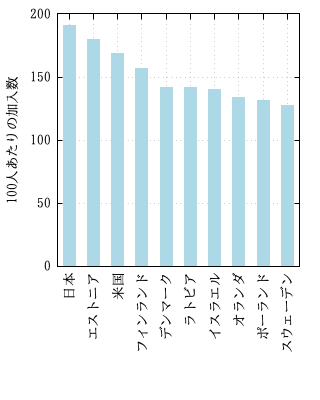
\includegraphics{fig21.png}
     \caption{図1:光ファイバー回線の加入者数(100人あたり)}\label{fig:ランキング}
\end{figure}
% \begin{figure}[htbp]
% \end{figure}
% で囲み
% \caption{}
% で図のタイトルを入れる.
% \label{}
% を使って図番号が参照できるようにする
% また,
% \centering
% で図が中央に来るようにする

% ーーー
\section{デジタル競争力ランキング}
国際経営開発研究所(IMD)の調査図\cite{imd}によると、
日本のデジタル競争力のランキングは表\ref{tbl:デジタル}に示すように、
調査対象の64カ国中、総合で28位、準備分野で27位となっている。
% 節見出し(2)

% 本文(2)

% 表の挿入
\begin{table}[htbp]
    \centering
    \caption{デジタル競争力ランキング(64カ国中}
    \label{tbl:デジタル}
    \begin{tabular}{|c|c|c|}
        \hline
        国  & 総合 & 準備 \\
        \hline
        米国 & 1位 & 1位 \\
        \hline
        香港 & 2位 & 10位 \\
        \hline
        スウェーデン & 3位 & 6位 \\
        \hline
        デンマーク & 4位 & 2位 \\
        \hline
        シンガポール & 5位 & 11位 \\
        \hline
        \hline
        韓国 & 12位 & 5位 \\
        \hline
        中国 & 15位 & 17位 \\
        \hline
        \hline
        日本 & 28位 & 27位 \\
        \hline
    \end{tabular}
\end{table}
% \end{tabular}    
% による表の記述を 
% \begin{table}[htbp]
% \end{table}
% で囲み
% \caption{}
% で表のタイトルを入れる.
% \label{}
% を使って表番号が参照できるようにする
% また,
% \centering
% で表が中央に来るようにする

% ーーー
\section{考察}
\begin{itemize}
    \item 米国がデジタルランキング1位にいる。そのことから今後、米国はより発展していくと感じる。
    
    \item 日本はブロードバンドでは1位であるが、デジタル競争力ランキングでは下の方であるため、これはデジタルだけではなく
    他の業界にも力を入れているからではないかと考えられる。
    
\end{itemize}
% 見出し(3)
% 考察
%
% \begin{itemize}
% \end{itemize}
% を使って箇条書きで記述する

% ここに参考文献が入る
%
\bibliographystyle{junsrt}
\bibliography{exercise.bib}

\end{document}